%!TEX root = ../thesis.tex

%%%%%%%%%%%%%%%%%%%%%%%%%
% Object reconstruction %
%%%%%%%%%%%%%%%%%%%%%%%%%
\message{^^J ^^J OBJECTS ^^J ^^J}
\newchap{Object \& Event Reconstruction} \label{sec:objects}
% https://twiki.cern.ch/twiki/bin/viewauth/CMS/Internal/PubDetector detector lines

%particularly
The lifetimes of particles like the Higgs, {\PW}, and {\PZ} bosons are extremely short ($\tau<10^{-20}\unit{s}$) and they decay shortly after their creation in pp collisions. Even if they have a large momentum, which increases their lifetime in the lab frame due to time dilation, they will travel a negligible distance, never reaching the pixel detector.

As the heaviest lepton, with a mass of $m_\PGt = 1.776\GeV$, a $\PGt$ lepton can decay not just to electrons and muons, but also to lighter hadrons. In each $\PGt$ decay, there will be at least one neutrino carrying away some momentum. %from the 

Except for the weakly interacting neutrinos, each of the final state particles mentioned above interacts with the detector in some special way.
This chapter is therefore devoted to describing how pp collision events and physics objects are reconstructed from data collected by the CMS detector and identified with dedicated algorithms.
A separate chapter will be dedicated to $\PGt$ leptons that decay to hadrons ($\tauh$), as their complex reconstruction builds on the techniques described in this chapter, and because I was involved with their reconstruction and identification in CMS.


%%%%%%%%%%%%%%%%%%%%%
%   PID PRINCIPLES  %
%%%%%%%%%%%%%%%%%%%%%
\section{Principles of particle identification} \label{sec:PID}

% FIGURE: Particle lifetimes
%!TEX root = ../thesis.tex


% FIGURE: Mass vs. lifetime
% https://www.sciencedirect.com/science/article/pii/S0146641019300109
\begin{figure*}[p!]
  \centering %\vspace{-6mm}
  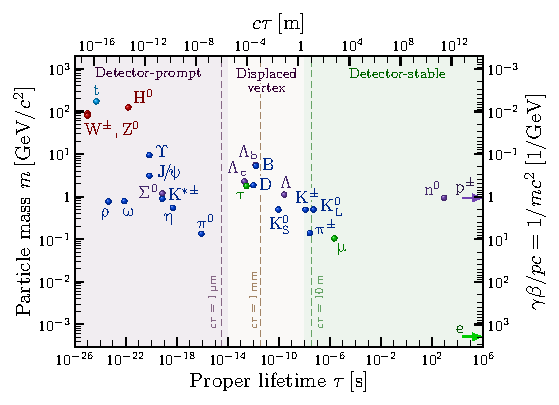
\includegraphics[width=10.5cm]{fig/objects/SM_particles_masses.pdf}
  \vspace{-2mm}
  \caption{
Plot of the mass versus lifetime $\tau$ of many composite and fundamental SM particles.
The decay length is given by $L=\gamma\beta c\tau$, with $\gamma\beta=p/mc$.
Adapted from Ref.~\cite{branching_fractions_fig}.
%Adapted from Ref.~\cite{lifetime_plot}.
  } \label{fig:lifetime}
\end{figure*}

% FIGURE: Particle identification
%!TEX root = ../thesis.tex

% FIGURE: PID principles
\begin{figure*}[p!]
  %\vspace{-3mm}
  \centering
  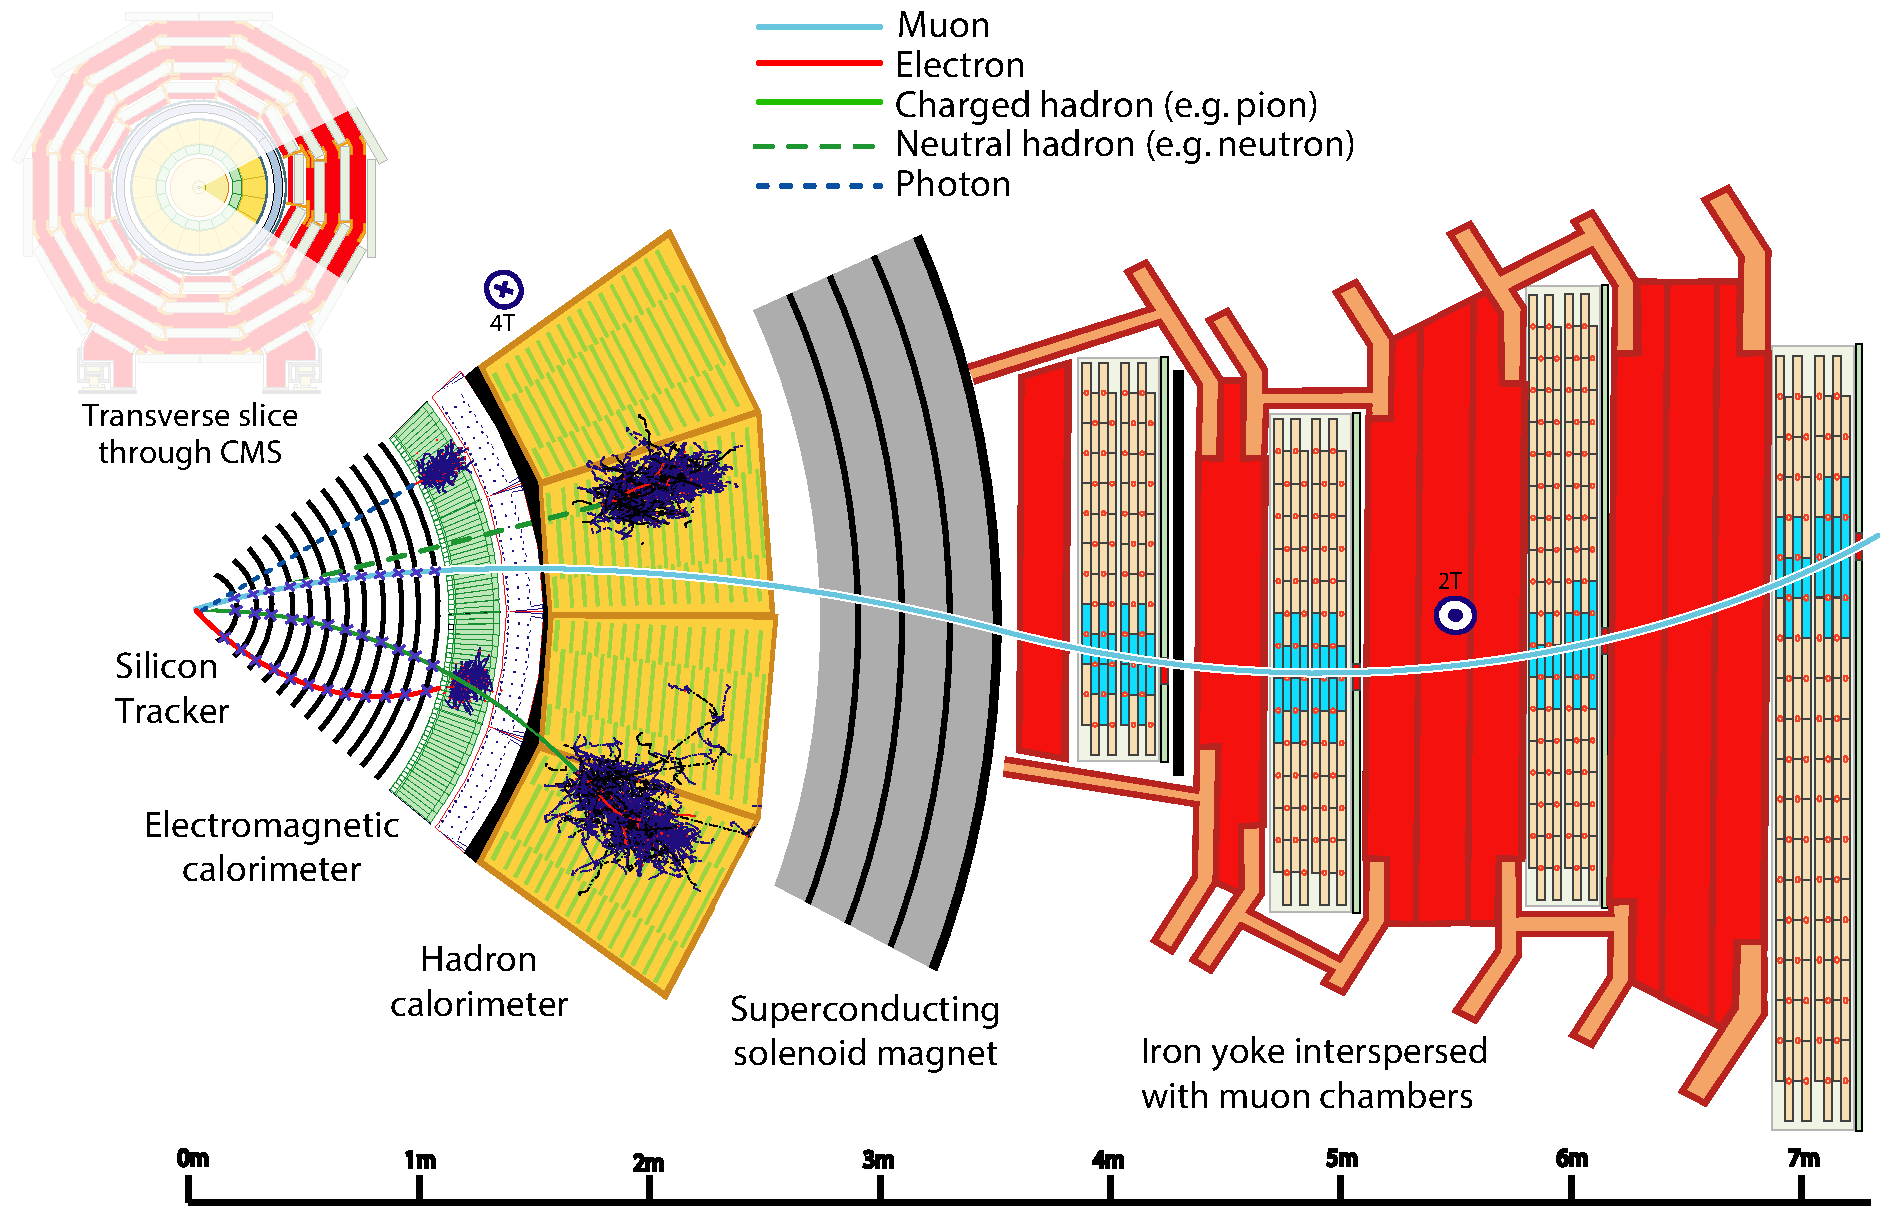
\includegraphics[width=0.92\textwidth]{fig/detector/CMS_detector_PID_edit.pdf}
  \caption{
Particles in the CMS detector.
Adapted from from~\cite{CMS_PID}. % David Barney.
  } \label{fig:PID}
  %\vspace{-3mm}
\end{figure*}


Figure~\ref{fig:lifetime} compares the lifetime, dividing them in different regions of stability in the context of the CMS experiment.
Each of these particles has a unique set of properties that leave a characteristic signal in one or more of the subdetector, as illustrated in \Fig{fig:PID}.


The top quark decays almost exclusively to a bottom quark and a $\PW$ boson instead of fragmenting into jets like the other quarks~\cite{BR_tt}.
The top's lifetime of $\tau\approx5\times10^{-25}\unit{s}$ is shorter than the time scale for fragmentation, which is around $10^{-24}\unit{s}$ (or equivalently, a distance scale of about $1\unit{fm}$)~\cite{hadronization_timescale1,hadronization_timescale2}.

Bottom quarks produced in high-energy collisions form $\PB$ hadrons that have typical lifetimes of $\tau\sim1.5\unit{ps}$. This is long enough for them to travel a measurable distance of the order of a few millimeters before decaying and creating a jet known as a \emph{b jet}. This can therefore create a \emph{secondary vertex} that is displaced from its production vertex, which CMS's tracking algorithm can reconstruct.

As \Fig{fig:lifetime} shows, $\PGt$ leptons and charmed hadrons are also capable of creating secondary vertices, although each of their decays tend to have a different topology, providing us with some efficiency for distinguishing them with identification algorithms.


%%%%%%%%%%%%%%%%%%%%%
%   PARTICLE-FLOW   %
%%%%%%%%%%%%%%%%%%%%%
\section{Particle-flow algorithm} \label{sec:PF}
The particle-flow (PF) algorithm~\cite{PF1,PF2017} fully reconstructs the event of a pp collision with an optimized combination of all measurements of the CMS subsystems.

Tracks in the inner tracker or muon system are iteratively built from hits, using the \emph{Kalman-filter} (KF) \emph{technique}~\cite{CMS_track_reco_2006,Kalman_filtering}.


%%%%%%%%%%%%%%%%%%%%%%
%   PRIMARY VERTEX   %
%%%%%%%%%%%%%%%%%%%%%%
\section{Primary vertex} \label{sec:PV}
The algorithm locates primary vertices (PVs) of $\Pp\Pp$ collisions.
The tracks are clustered using the \emph{deterministic annealing algorithm}~\cite{deterministic_annealing}.
Finally, candidate vertices are fitted using an \emph{adaptive vertex fitter}~\cite{vertex_fitting}.
The PV with the largest sum of momenta is assumed to be the vertex of the hard scattering process~\cite{CMS_vertex,PF2017,CMS_vertex_phase2}.


%%%%%%%%%%%%%%%%%
%   ELECTRONS   %
%%%%%%%%%%%%%%%%%
\section{Electrons} \label{sec:electron}

Electrons are reconstructed by associating a track in the inner tracker to clusters of energy deposits in the ECAL.
% tracks
Candidate tracks are refitted with the \emph{Gaussian sum filter} (GSF)~\cite{GSF}.
% shower
The ECAL clusters are recombined into a so-called \emph{supercluster}.
The resolution is documented in Ref.~\cite{CMS_electron_2021,CMS_electron_calibration_2016}.

% ID
The reconstruction and identification of electrons, as well as high-energy photons, are discussed in more detail in Refs.~\cite{CMS_electron} and~\cite{CMS_electron_2021}.

The \emph{relative isolation} for electrons is computed with the so-called \emph{rho-effective-area method}~\cite{PU_substraction}:
\begin{equation} \label{eq:iso_ele}
  \Irel^{\Pe} \defeq
    \frac{\sum_\text{charged} \PT + \max\left( 0, \sum_\text{neutral} \ET
                                  - \rho A_\text{eff} \right )}{\pt^{\Pe}}. 
\end{equation}


%%%%%%%%%%%%%
%   MUONS   %
%%%%%%%%%%%%%
\section{Muons} \label{sec:muon}
Muon candidates in CMS are reconstructed as \emph{standalone muons}, \emph{tracker muons}, and/or \emph{global muons}~\cite{CMS_muon_2018}.

% RELATIVE ISOLATION
The relative isolation of a muon is defined with the so-called \emph{$\Delta\beta$-corrections}:
\begin{equation}\label{eq:iso_mu}
  \Irel^{\PGm} \defeq
    \frac{\sum_\text{charged} \pt + \max\left( 0, \sum_\text{neutral} \ET
                                  - \Delta\beta \sum_\text{charged, PU} \pt \right )}{\pt^{\PGm}}.
\end{equation}



%%%%%%%%%%%%
%   JETS   %
%%%%%%%%%%%%
\section{Jets}\label{sec:jets}

% https://arxiv.org/abs/1706.04965
Jets are reconstructed with a clustering algorithm.
The jet properties must be \emph{infrared safe} and \emph{collinear safe}.
% anti-kT
The \emph{anti-$\kt$} (AK) \emph{algorithm} utilizes the metric
\begin{equation} \label{eq:antikT}
  d_{ij} = \min\left(p_\text{T,i}^{-2},p_\text{T,j}^{-2}\right)\frac{\Delta R^2_{ij}}{\Delta R_y^2},
\end{equation}
where $\Delta R_y=\sqrt{\Delta y^2+\Delta\phi^2}$ is the distance in $(y,\phi)$-space with the \emph{rapidity}
\begin{equation} \label{eq:rapidity}
  y \defeq \frac{1}{2}\ln\left(\frac{E+p_z}{E-p_z}\right).
\end{equation}
If a cluster $i$ of combined objects satisfies
\begin{equation} \label{eq:antikT_cut}
  d_{ij} > d_{i\text{B}} = p_\text{T,i}^{-2},
\end{equation}
the algorithm defines it to be a jet and removes its PF candidates from consideration in clustering subsequent jets~\cite{PF2017,antikT}.
The AK algorithm is implemented in the \FASTJET library~\cite{fastjet1,fastjet2}, and CHS is used to remove charged PF candidates not associated with the PV of the hard interaction.

% JEC
The CMS Collaboration determines \emph{jet energy corrections} (JECs) in several steps, which are explained in detail in Ref.~\cite{CMS-JME-10-011}.
Additionally, the jet energy and \emph{jet energy resolution} (JER) of jets in simulation are corrected to obtain better agreement between simulation and data.

% JET ID
Genuine jets are distinguished from pileup jets with the identification algorithm~\cite{jetPUID}.
Spurious jet-like features that originate from isolated noise patterns in certain HCAL regions with identification~\cite{jetID_2016}.


%%%%%%%%%%%%%
%   B TAG   %
%%%%%%%%%%%%%
\section{Bottom quark identification} \label{sec:btagging}

% FIGURE: B TAGGING ILLUSTRATION
%!TEX root = ../thesis.tex

% FIGURE: PID
\begin{figure*}[t!]
  %\vspace{-6mm}
  \centering
  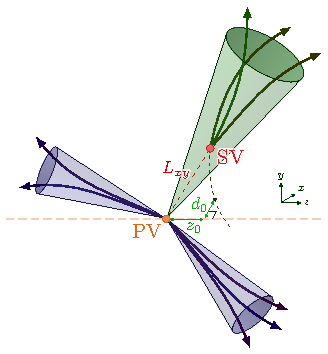
\includegraphics[width=0.33\textwidth]{fig/objects/jet_btag.pdf}
  %\vspace{-2mm}
  \caption{
B-tagging.
  } \label{fig:btagging}
  %\vspace{-8mm}
\end{figure*}


The \DeepCSV algorithm~\cite{btag_deepCSV,btag_2018} for b tagging jets. \DeepCSV is a deep neural network (DNN) with four hidden layers that is an extension of the combined secondary vertex (CSV) algorithm~\cite{btag_deepCSV,btag_2018}.


%%%%%%%%%%%
%   MET   %
%%%%%%%%%%%
% https://twiki.cern.ch/twiki/bin/view/CMSPublic/WorkBookMetAnalysis#7_7_6_MET_Corrections
\section{Missing transverse energy}\label{sec:met}

% FIGURE: MET
%!TEX root = ../thesis.tex

% FIGURE: MET
\begin{figure*}[t]
  %\vspace{-6mm}
  \centering
  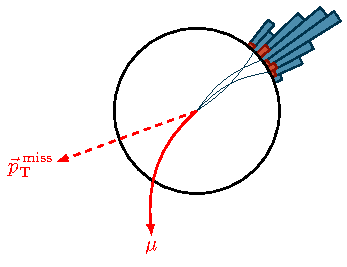
\includegraphics[width=0.39\textwidth]{fig/objects/transverse_plane.pdf}
  %\vspace{-2mm}
  \caption{
Illustration of missing transverse energy (MET) with a muon track (red), and energy deposits in the calorimeters.
  } \label{fig:MET}
  %\vspace{-2mm}
\end{figure*}


The vectorially sum of all particles gives the missing momentum
\begin{equation} \label{eq:MET}
  \ptvecmiss = - \sum_{\text{i}}\myvec{p}_\text{T}^{\,i}.
\end{equation}
This vector, or its length, is often referred to as the \emph{missing transverse momentum}, or \emph{missing transverse energy} (MET).
Several corrections are applied~\cite{PF2017}.
More details can be found in Refs.~\cite{CMS-PAS-JME-16-004} and~\cite{CMS-PAS-JME-17-001}. 

